% THIS DOCUMENT IS TAILORED TO REQUIREMENTS FOR SCIENTIFIC COMPUTING.  IT SHOULDN'T
% BE USED FOR NON-SCIENTIFIC COMPUTING PROJECTS
\documentclass[12pt]{article}

\usepackage{amsmath, mathtools}
\usepackage{amsfonts}
\usepackage{amssymb}
\usepackage{graphicx}
\graphicspath{{../assets}} % Bring in the assets

\usepackage{colortbl}
\usepackage{xr}
\usepackage{hyperref}
\usepackage{longtable}
\usepackage{xfrac}
\usepackage{tabularx}
\usepackage{float}
\usepackage{siunitx}
\usepackage{booktabs}
\usepackage{caption}
\usepackage{pdflscape}
\usepackage{afterpage}

\usepackage{tikz}
\usepackage{varwidth}
\usetikzlibrary{shapes,arrows,cd,babel,arrows.meta,graphs,graphdrawing}
\usegdlibrary {layered}

% Credit to Gabriel Devenyi for this bibliography cfg:
% github.com/gdevenyi/mcmaster.latex
\usepackage[ style=numeric-comp, backend=biber, sorting=none, backref=true,
  maxnames=99, alldates=iso, seconds=true ]{biblatex} % bibliography
\addbibresource{../references.bib}

%\usepackage{refcheck}

\hypersetup{
    bookmarks=true,         % show bookmarks bar?
    colorlinks=true,       % false: boxed links; true: colored links
    linkcolor=red,          % color of internal links (change box color with linkbordercolor)
    citecolor=green,        % color of links to bibliography
    filecolor=magenta,      % color of file links
    urlcolor=cyan           % color of external links
}
\usepackage{cleveref}


%% Comments

\usepackage{color}

\newif\ifcomments\commentstrue %displays comments
%\newif\ifcomments\commentsfalse %so that comments do not display

\ifcomments
\newcommand{\authornote}[3]{\textcolor{#1}{[#3 ---#2]}}
\newcommand{\todo}[1]{\textcolor{red}{[TODO: #1]}}
\else
\newcommand{\authornote}[3]{}
\newcommand{\todo}[1]{}
\fi

\newcommand{\wss}[1]{\authornote{blue}{SS}{#1}} 
\newcommand{\plt}[1]{\authornote{magenta}{TPLT}{#1}} %For explanation of the template
\newcommand{\an}[1]{\authornote{cyan}{Author}{#1}}

%% Common Parts

\newcommand{\progname}{BeamBending}
\newcommand{\authname}{\small{\textit{Team Drasil}}\\Jason Balaci}
\newcommand{\authinitials}{JB}

\usepackage{hyperref}
\hypersetup{colorlinks=true, linkcolor=blue, citecolor=blue, filecolor=blue,
            urlcolor=blue, unicode=false}
\urlstyle{same}

%%%%%%%%%%%%%%%%%%%%%%%%%%%%%%%%%%%%%%%%%%%%%%%%%%%%%%%%%%%%%%%%%%%%%%%%%%%%%%%
% QUESTION DIRECTED WRITING
\ifshowwritingdirectives
  \newenvironment{writingdirectives}{\begin{mdwritingdirectives}\centering\textbf{Writing Directives}\begin{itemize}}{\end{itemize}\end{mdwritingdirectives}}
\else
  \excludecomment{writingdirectives}
\fi

\newcommand{\wqanswer}[1]{\textit{#1}}

%%%%%%%%%%%%%%%%%%%%%%%%%%%%%%%%%%%%%%%%%%%%%%%%%%%%%%%%%%%%%%%%%%%%%%%%%%%%%%%
% SPACING OPTIONS
\newcommand{\thesisForceSingleSpacing}{\singlespacing}
\newcommand{\thesisForceDoubleSpacing}{\doublespacing}

%%%%%%%%%%%%%%%%%%%%%%%%%%%%%%%%%%%%%%%%%%%%%%%%%%%%%%%%%%%%%%%%%%%%%%%%%%%%%%%
% CASE STUDIES
\newcommand{\caseStudy}[1]{\ACL{#1} (\textit{\acs{#1}})}

%%%%%%%%%%%%%%%%%%%%%%%%%%%%%%%%%%%%%%%%%%%%%%%%%%%%%%%%%%%%%%%%%%%%%%%%%%%%%%%
% JUDGMENTS

\newcommand{\newrule}[2]{\begin{equation} \infer{#2}{#1} \end{equation}} % Adds to automatically numbered equations
\newcommand{\newlblrule}[3]{\begin{equation} \infer{#2}{#1} \label{#3}\end{equation}} % Adds to automatically numbered equations, with a label
\newcommand{\exampleRule}[2]{\[ \infer{#2}{#1} \]} % Does not add a number to equations

\newcommand{\Tau}{\mathrm{T}}
\newcommand{\ty}[1]{\texttt{#1} : \tau}

\newcommand{\ofTy}[2]{#1 : \texttt{#2}}

\newcommand{\numericTy}[1]{\ofTy{#1}{\texttt{Numerics($\Tau$)}}}
\newcommand{\negNumericTy}[1]{\ofTy{#1}{\texttt{NumericsWithNegation($\Tau$)}}}

%%%%%%%%%%%%%%%%%%%%%%%%%%%%%%%%%%%%%%%%%%%%%%%%%%%%%%%%%%%%%%%%%%%%%%%%%%%%%%%
% MATH

\newcommand{\bb}[1]{\mathbb{#1}}

%%%%%%%%%%%%%%%%%%%%%%%%%%%%%%%%%%%%%%%%%%%%%%%%%%%%%%%%%%%%%%%%%%%%%%%%%%%%%%%
% SYNTAX CHARTS
\newcommand{\startSyntaxTable}{\begin{longtable}{ r c c l c l }}
\newcommand{\newsyntaxRow}[5]{#1 & \( #2 \) & $::=$ & \texttt{#3} & $#4$ & #5 \\}
\newcommand{\syntaxRow}[3]{& & $\vert$ & \texttt{#1} & $#2$ & #3 \\}
\newcommand{\closeSyntaxTable}{\end{longtable}}

%%%%%%%%%%%%%%%%%%%%%%%%%%%%%%%%%%%%%%%%%%%%%%%%%%%%%%%%%%%%%%%%%%%%%%%%%%%%%%%
% Footnotes that only show "when compiling for printing"

\ifcompilingforprinting
  \newcommand{\printOnlyFootnote}[1]{\footnote{#1}}
  \newcommand{\printOnlyFootnoteText}[1]{\footnotetext{#1}}
  \newcommand{\printOnlyFootnoteMark}{\footnotemark}
\else
  \newcommand{\printOnlyFootnote}[1]{}
  \newcommand{\printOnlyFootnoteText}[1]{}
  \newcommand{\printOnlyFootnoteMark}{}
\fi

%%%%%%%%%%%%%%%%%%%%%%%%%%%%%%%%%%%%%%%%%%%%%%%%%%%%%%%%%%%%%%%%%%%%%%%%%%%%%%%
% Portable HREFs

% Common variant
\newcommand{\porthref}[2]{\href{#2}{#1}\printOnlyFootnote{\url{#2}}}
% Custom URLs
\newcommand{\porthreft}[3]{\href{#3}{#1}\printOnlyFootnote{\href{#3}{#2}}}
% Inside of some environments, footnote marks aren't registered properly, so we
% need to manually write the "text" part
\newcommand{\porthreftm}[2]{\href{#2}{#1\printOnlyFootnoteMark}}

%%%%%%%%%%%%%%%%%%%%%%%%%%%%%%%%%%%%%%%%%%%%%%%%%%%%%%%%%%%%%%%%%%%%%%%%%%%%%%%
% TODOs

% Generic Inlined TODOs
\newcommand{\intodo}[1]{\todo[inline]{#1}}

% Unimportant TODOs for "later" (i.e., finishing touches or changes immediately before submission)
\newcommand{\latertodo}[1]{\todo[backgroundcolor=Cyan]{\textit{Later}: #1}}

% "Important" TODOs
\newcommand{\imptodo}[1]{\todo[inline,backgroundcolor=Red]{\textbf{Important}: #1}}

% "Easy" TODOs
\newcommand{\easytodo}[1]{\todo[inline,backgroundcolor=SeaGreen]{\textit{Easy}: #1}}
\newcommand{\eztodo}[1]{\easytodo{#1}}

% "Tedious" TODOs
\newcommand{\tedioustodo}[1]{\todo[inline,backgroundcolor=PineGreen]{\textit{Needs time}: #1}}

% "Question" TODO Notes
\newcounter{todonoteQuestionsCtr}
\newcommand{\questiontodo}[1]{\stepcounter{todonoteQuestionsCtr}\todo[backgroundcolor=Lavender]{\textbf{Q \#\thetodonoteQuestionsCtr{}}: #1}}
\newcommand{\qtodo}[1]{\questiontodo{#1}}


%%%%%%%%%%%%%%%%%%%%%%%%%%%%%%%%%%%%%%%%%%%%%%%%%%%%%%%%%%%%%%%%%%%%%%%%%%%%%%%
% Haskell snippet
\newenvironment{code}{\captionsetup{type=listing,skip=14pt}}{}
\SetupFloatingEnvironment{listing}{name=Source Code, listname=List of Source Codes}
\crefname{listing}{source code}{source codes}
\Crefname{listing}{Source Code}{Source Codes}

\newenvironment{haskell}[3]
  {\VerbatimEnvironment\thesisForceSingleSpacing{}\begin{code}\captionof{listing}[#1]{\protect\porthreftm{#1}{#3}}\printOnlyFootnoteText{\protect\url{#3}}\label{lst:#2}\begin{minted}[frame=lines,framerule=2pt,breaklines]{haskell}}
  {\end{minted}\end{code}\thesisSpacing{}}

\newenvironment{codeSnippet}[4]
  {\VerbatimEnvironment\thesisForceSingleSpacing{}\begin{code}\captionof{listing}[#2]{\protect\porthreftm{#2}{#4}}\printOnlyFootnoteText{\protect\url{#4}}\label{lst:#3}\begin{minted}[frame=lines,framerule=2pt,breaklines]{#1}}
  {\end{minted}\end{code}\thesisSpacing{}}

\newenvironment{pseudohaskell}[2]
  {\VerbatimEnvironment\thesisForceSingleSpacing{}\begin{code}\captionof{listing}{Pseudocode: #1}\label{lst:#2}\begin{minted}[frame=lines,framerule=2pt,breaklines]{haskell}}
  {\end{minted}\end{code}\thesisSpacing{}}

\newenvironment{pseudocode}[3]
  {\VerbatimEnvironment\thesisForceSingleSpacing{}\begin{code}\captionof{listing}{Pseudocode: #2}\label{lst:#3}\begin{minted}[frame=lines,framerule=2pt,breaklines]{#1}}
  {\end{minted}\end{code}\thesisSpacing{}}

\newcommand{\inlineHs}[1]{\mintinline{haskell}|#1|}
\newcommand{\inlineCode}[2]{\mintinline{#1}|#2|}


% For easy change of table widths
\newcommand{\colZwidth}{1.0\textwidth}
\newcommand{\colAwidth}{0.13\textwidth}
\newcommand{\colBwidth}{0.82\textwidth}
\newcommand{\colCwidth}{0.1\textwidth}
\newcommand{\colDwidth}{0.05\textwidth}
\newcommand{\colEwidth}{0.8\textwidth}
\newcommand{\colFwidth}{0.17\textwidth}
\newcommand{\colGwidth}{0.5\textwidth}
\newcommand{\colHwidth}{0.28\textwidth}

% Used so that cross-references have a meaningful prefix
\newcounter{defnum} %Definition Number
\newcommand{\dthedefnum}{GD\thedefnum}
\newcommand{\dref}[1]{GD\ref{#1}}
\newcounter{datadefnum} %Datadefinition Number
\newcommand{\ddthedatadefnum}{DD\thedatadefnum}
\newcommand{\ddref}[1]{DD\ref{#1}}
\newcounter{theorynum} %Theory Number
\newcommand{\tthetheorynum}{T\thetheorynum}
\newcommand{\tref}[1]{T\ref{#1}}
\newcounter{tablenum} %Table Number
\newcommand{\tbthetablenum}{T\thetablenum}
\newcommand{\tbref}[1]{TB\ref{#1}}
\newcounter{assumpnum} %Assumption Number
\newcommand{\atheassumpnum}{P\theassumpnum}
\newcommand{\aref}[1]{A\ref{#1}}
\newcounter{goalnum} %Goal Number
\newcommand{\gthegoalnum}{P\thegoalnum}
\newcommand{\gsref}[1]{GS\ref{#1}}
\newcounter{instnum} %Instance Number
\newcommand{\itheinstnum}{IM\theinstnum}
\newcommand{\iref}[1]{IM\ref{#1}}
\newcounter{reqnum} %Requirement Number
\newcommand{\rthereqnum}{P\thereqnum}
\newcommand{\rref}[1]{R\ref{#1}}
\newcounter{nfrnum} %NFR Number
\newcommand{\rthenfrnum}{NFR\thenfrnum}
\newcommand{\nfrref}[1]{NFR\ref{#1}}
\newcounter{lcnum} %Likely change number
\newcommand{\lthelcnum}{LC\thelcnum}
\newcommand{\lcref}[1]{LC\ref{#1}}

\usepackage{fullpage}

\newcommand{\deftheory}[9][Not Applicable]
{
\newpage
\noindent \rule{\textwidth}{0.5mm}

\paragraph{RefName: } \textbf{#2} \phantomsection 
\label{#2}

\paragraph{Label:} #3

\noindent \rule{\textwidth}{0.5mm}

\paragraph{Equation:}

#4

\paragraph{Description:}

#5

\paragraph{Notes:}

#6

\paragraph{Source:}

#7

\paragraph{Ref.\ By:}

#8

\paragraph{Preconditions for \hyperref[#2]{#2}:}
\label{#2_precond}

#9

\paragraph{Derivation for \hyperref[#2]{#2}:}
\label{#2_deriv}

#1

\noindent \rule{\textwidth}{0.5mm}

}

\begin{document}

%%%%%%%%%%%%%%%%%%%%%%%%%%%%%%%%%%%%%%%%%%%%%%%%%%%%%%%%%%%%%%%%%%%%%%%%%%%%%%%
% Title
%%%%%%%%%%%%%%%%%%%%%%%%%%%%%%%%%%%%%%%%%%%%%%%%%%%%%%%%%%%%%%%%%%%%%%%%%%%%%%%

\title{Software Requirements Specification for \progname: examining a beam bending under load.}
\author{\authname}
\date{\today}

\maketitle

~\newpage

\pagenumbering{roman}

\tableofcontents

~\newpage

%%%%%%%%%%%%%%%%%%%%%%%%%%%%%%%%%%%%%%%%%%%%%%%%%%%%%%%%%%%%%%%%%%%%%%%%%%%%%%%
% Revision History
%%%%%%%%%%%%%%%%%%%%%%%%%%%%%%%%%%%%%%%%%%%%%%%%%%%%%%%%%%%%%%%%%%%%%%%%%%%%%%%

\section*{Revision History}

\begin{tabularx}{\textwidth}{p{3cm}p{2cm}X}
    \toprule {\bf Date} & {\bf Version} & {\bf Notes}                      \\
    \midrule
    Jan. 25, 2023       & 0.0.0         & Template imported.               \\
    Jan. 25, 2023       & 0.1.0         & Preliminary information added.   \\
    Jan. 25, 2023       & 0.1.1         & Table of units added.            \\
    Jan. 25, 2023       & 0.1.2         & Table of symbols added.          \\
    Jan. 25, 2023       & 0.1.3         & Refining above tables.           \\
    Jan. 25, 2023       & 0.2.0         & Refined introduction.            \\
    Jan. 25, 2023       & 0.3.0         & Refining GSD, SSD, TMs, and IMs. \\
    \bottomrule
\end{tabularx}


\noindent \plt{Advice on using the template:
    \begin{itemize}
        \item Difference between physical and software constraints
        \item Properties of a correct solution means \emph{additional} properties, not
              a restating of the requirements (may be ``not applicable'' for your problem).
              If you have a table of output constraints, then these are properties of a
              correct solution.
        \item Assumptions have to be invoked somewhere
        \item ``Referenced by'' implies that there is an explicit reference
        \item Think of traceability matrix, list of assumption invocations and list of
              reference by fields as automatically generatable
        \item If you say the format of the output (plot, table etc), then your
              requirement could be more abstract
    \end{itemize}
}

~\newpage

%%%%%%%%%%%%%%%%%%%%%%%%%%%%%%%%%%%%%%%%%%%%%%%%%%%%%%%%%%%%%%%%%%%%%%%%%%%%%%%
% Reference Material
%%%%%%%%%%%%%%%%%%%%%%%%%%%%%%%%%%%%%%%%%%%%%%%%%%%%%%%%%%%%%%%%%%%%%%%%%%%%%%%

\section{Reference Material}

This section records information for easy reference.

\subsection{Table of Units}

Throughout this document SI (Syst\`{e}me International d'Unit\'{e}s) is employed
as the unit system.  In addition to the basic units, several derived units are
used as described below.  For each unit, the symbol is given followed by a
description of the unit and the SI name. ~\newline

\begin{center}
    \renewcommand{\arraystretch}{1.2}
    \noindent \begin{tabular}{l l l}
        \toprule
        \textbf{symbol} & \textbf{unit} & \textbf{SI} \\
        \midrule
        \si{\metre}     & length        & metre       \\
        \si{\gram}      & mass          & gram        \\
        \si{\pascal}    & pressure      & pascal      \\
        \si{\radian}    & angle         & radian      \\
        \si{\newton}    & force         & newton      \\
        \bottomrule
    \end{tabular}\\
\end{center}

\noindent{}Note that we will also often use:

\begin{itemize}

    \item ``gigapascals'' (a unit of pressure, denoted by \si{\giga\pascal},
          where \(\si{\giga\pascal}=10^{9}\si{\pascal}\)),

    \item ``kilograms'' (a unit of mass, \si{\kilogram}, where
          \(\si{\kilogram}=10^{3}\si{\gram}\)),

    \item ``kilonewtons'' (a unit of force, denoted by \si{\kilo\newton}, where
          \(\si{\kilo\newton}=10^{3}\si{\newton}\)), and

    \item ``millimetres'' (a unit of length, denoted by \si{\milli\metre}, where
          \(\si{\milli\metre}=10^{-5}\si{\metre}\)).

\end{itemize}

\subsection{Table of Symbols}

The table that follows summarizes the symbols used in this document along with
their units.  The choice of symbols was made to be consistent with the heat
transfer literature and with existing documentation for solar water heating
systems.  The symbols are listed in alphabetical order.

\renewcommand{\arraystretch}{1.2}
\noindent
\begin{longtable*}{l l p{12cm}}
    \toprule
    \textbf{symbol} & \textbf{unit} & \textbf{description}\\
    \midrule
    \(L\) & \si{\metre} & abstract length of the beam \\
    \(E\) & \si{\giga\pascal} & abstract Young's modulus (beam material modulus of elasticity) \\
    \(I\) & \(\si{\metre{}}^{4}\) & abstract moment of inertia \\
    \(L_{B}\) & \si{\metre} & user-defined length of the beam \\
    \(E_{B}\) & \si{\giga\pascal} & user-defined Young's modulus (beam material modulus of elasticity) \\
    \(I_{B}\) & \(\si{\metre{}}^{4}\) & user-defined moment of inertia of a cross-section of the beam \\
    \(n\) & \textemdash{} & user-defined number of (imposed force, deflection) samples to take along the beam \\
    \(f(x)\) & \si{\kilo\newton} & user-defined definition of the force of the load applied at a specific point along the beam \\
    \(x\) & \si{\metre} & distance of an arbitrary point along the beam, from the far left-side (at the pinned support) \\
    \(w(x)\) & \si{\kilo\newton} & hypothetical force of the load applied at a specific point along the beam \\
    \(\mathit{Pinned}\) & \si{\metre} & 1-dimensional position of the pinned support \\
    \(\mathit{Roller}\) & \si{\metre} & 1-dimensional position of the roller support \\
    \(R_{\mathit{Pinned}}\) & \si{\kilo\newton} & reaction of the pinned support under loaded beam \\
    \(R_{\mathit{Roller}}\) & \si{\kilo\newton} & reaction of the roller support under loaded beam \\
    \(\theta{}_{\mathit{Pinned}}\) & \si{\radian} & slope of the angle between the beam and the pinned support under load \\
    \(\theta{}_{\mathit{Roller}}\) & \si{\radian} & slope of the angle between the beam and the roller support under load \\
    \(y(x)\) & \si{\milli\metre} & deflection of the loaded beam at a specific point along it \\
    \(s\) & \si{\milli\metre} & loaded beam movement in the rightward direction of the roller support \\
    \(\vec{r}\) & \textemdash{} & $n+1$-dimensional vector of equally-spaced $(w(x),y(x))$ samples along the beam \\
    \bottomrule
\end{longtable*}

\subsection{Abbreviations and Acronyms}

\renewcommand{\arraystretch}{1.2}

\begin{center}
    \begin{tabular}{l l}
        \toprule
        \textbf{symbol} & \textbf{description}                \\
        \midrule
        A               & Assumption                          \\
        BVP             & Boundary Value Problem              \\
        DD              & Data Definition                     \\
        GD              & General Definition                  \\
        GS              & Goal Statement                      \\
        IM              & Instance Model                      \\
        LC              & Likely Change                       \\
        PS              & Physical System Description         \\
        R               & Requirement                         \\
        SRS             & Software Requirements Specification \\
        \progname{}     & Beam Bending                        \\
        TM              & Theoretical Model                   \\
        \bottomrule
    \end{tabular}
\end{center}

\subsection{Mathematical Notation}

Vector symbols will be represented using the ``arrow'' notation, where a
right-ward facing arrow is placed atop a symbol denoting a vector. For example,
\(\vec{v}\) is a vector symbol. Additionally, the standard ``tuple'' notation
will also be used to denote tuples.

\newpage

\pagenumbering{arabic}

%%%%%%%%%%%%%%%%%%%%%%%%%%%%%%%%%%%%%%%%%%%%%%%%%%%%%%%%%%%%%%%%%%%%%%%%%%%%%%%
% Introduction
%%%%%%%%%%%%%%%%%%%%%%%%%%%%%%%%%%%%%%%%%%%%%%%%%%%%%%%%%%%%%%%%%%%%%%%%%%%%%%%

\section{Introduction}

For any structure carrying load, beams are used to safely distribute the stress
of the load to the foundations of the structure. Unlike flooring in residential
homes, we expect the beds of industrial-strength mechanical tools and bridges
to, within reason, be vertically and horizontally flexible, reacting to imposed
load such that they may hold with minimal columns. \textit{Simply supported}
beams are one type of beam that are commonly found in bridges and beds of
machine tools. It is important to understand how beams will react under load or
else we risk damaging structures, floor bending (making inhabitants feel
unsafe), or damaging loads. We may use software to analyze the beams reaction
under various loading scenarios. We call the software that performs this,
``BeamBending.''

This document aims to develop a general scheme for understanding the reaction of
a simply supported beam to imposed load under simplified conditions. This
section aims to provide an overview of the Software Requirements Specification
(SRS) for the ``BeamBending'' problem, discussing the scope and purpose of the
work.

\subsection{Purpose of Document}

The purpose of this document is to provide the reader with a well-derived,
verifiable explanation of a solution to the ``beam bending'' problem. The
document provides sufficient information such that a related software artifact
may be constructed. The produced software artifact has an ``increased'' degree
of confidence in reliability and correctness by being traceable to and derived
by these defined software requirements specifications. As such, a large focus on
the development of this document is to have the domain knowledge captured and
adequately codified such that the origins of fragments of code may be verified,
up to development choices (e.g., language, tooling, etc.).

\subsection{Scope of Requirements} \label{ssec_scope}

The requirements analyze the ``problem'' (as defined in \autoref{Sec_pd}) and
related ``solution'' under the assumption of the Euler-Bernoulli Beam Theory
\cite{EulerBernoulliWiki} in a 2-dimensional space for a prismatic beam.

\subsection{Characteristics of Intended Reader} \label{sec_IntendedReader}

Readers of this document should at least have an understanding of:
\begin{itemize}
    \item at least a first-year university level physics concepts, such as
          ``force,'' ``mass,'' ``inertia,'' ``elasticity,'' and ``units,''
    \item first-year university level linear algebra and calculus concepts, such
          as derivatives, integration, continuous functions, and vectors.
\end{itemize}

However, it is preferred that users have at least a second-year university level
understand of physics and calculus concepts to confidently audit the derivation
of the instance models.

Should this document be used for non-trivial, non-educational purposes, this
document should strictly be read and used by those appropriately licensed and
well-versed in software and civil engineering.

\subsection{Organization of Document}

This document follows the SRS template as specified by Smith and Lai
\cite{SmithAndLai2005}. If you are already familiar with the SRS template, the
author's recommended, but not required, reading order is as follows:

\begin{itemize}
    \item \nameref{Sec_pd},
    \item \nameref{sssec_goals},
    \item \nameref{sec_IntendedReader},
    \item \nameref{ssec_scope},
    \item \nameref{sec_gsd},
    \item \nameref{sec_assumpt},
    \item \nameref{sec_ssd}, and, finally,
    \item \nameref{sec_instance} to \nameref{sec_theoretical}.
\end{itemize}

The other material is referential and may be read as needed.

\newpage

%%%%%%%%%%%%%%%%%%%%%%%%%%%%%%%%%%%%%%%%%%%%%%%%%%%%%%%%%%%%%%%%%%%%%%%%%%%%%%%
% General System Description
%%%%%%%%%%%%%%%%%%%%%%%%%%%%%%%%%%%%%%%%%%%%%%%%%%%%%%%%%%%%%%%%%%%%%%%%%%%%%%%

\section{General System Description} \label{sec_gsd}

This section provides general information about the system so that the next
section will be easier to digest. It identifies the interfaces between the
system and its environment, describes the user characteristics, and lists the
system constraints.

\subsection{System Context}

\plt{Your system context will include a figure that shows the abstract view of
    the software.  Often in a scientific context, the program can be viewed
    abstractly following the design pattern of Inputs $\rightarrow$ Calculations
    $\rightarrow$ Outputs.  The system context will therefore often follow this
    pattern.  The user provides inputs, the system does the calculations, and
    then provides the outputs to the user.  The figure should not show all of
    the inputs, just an abstract view of the main categories of inputs (like
    material properties, geometry, etc.).  Likewise, the outputs should be
    presented from an abstract point of view.  In some cases the diagram will
    show other external entities, besides the user.  For instance, when the
    software product is a library, the user will be another software program,
    not an actual end user. If there are system constraints that the software
    must work with external libraries, these libraries can also be shown on the
    System Context diagram. They should only be named with a specific library
    name if this is required by the system constraint.}

% \begin{figure}[h!]
%     \begin{center}
%         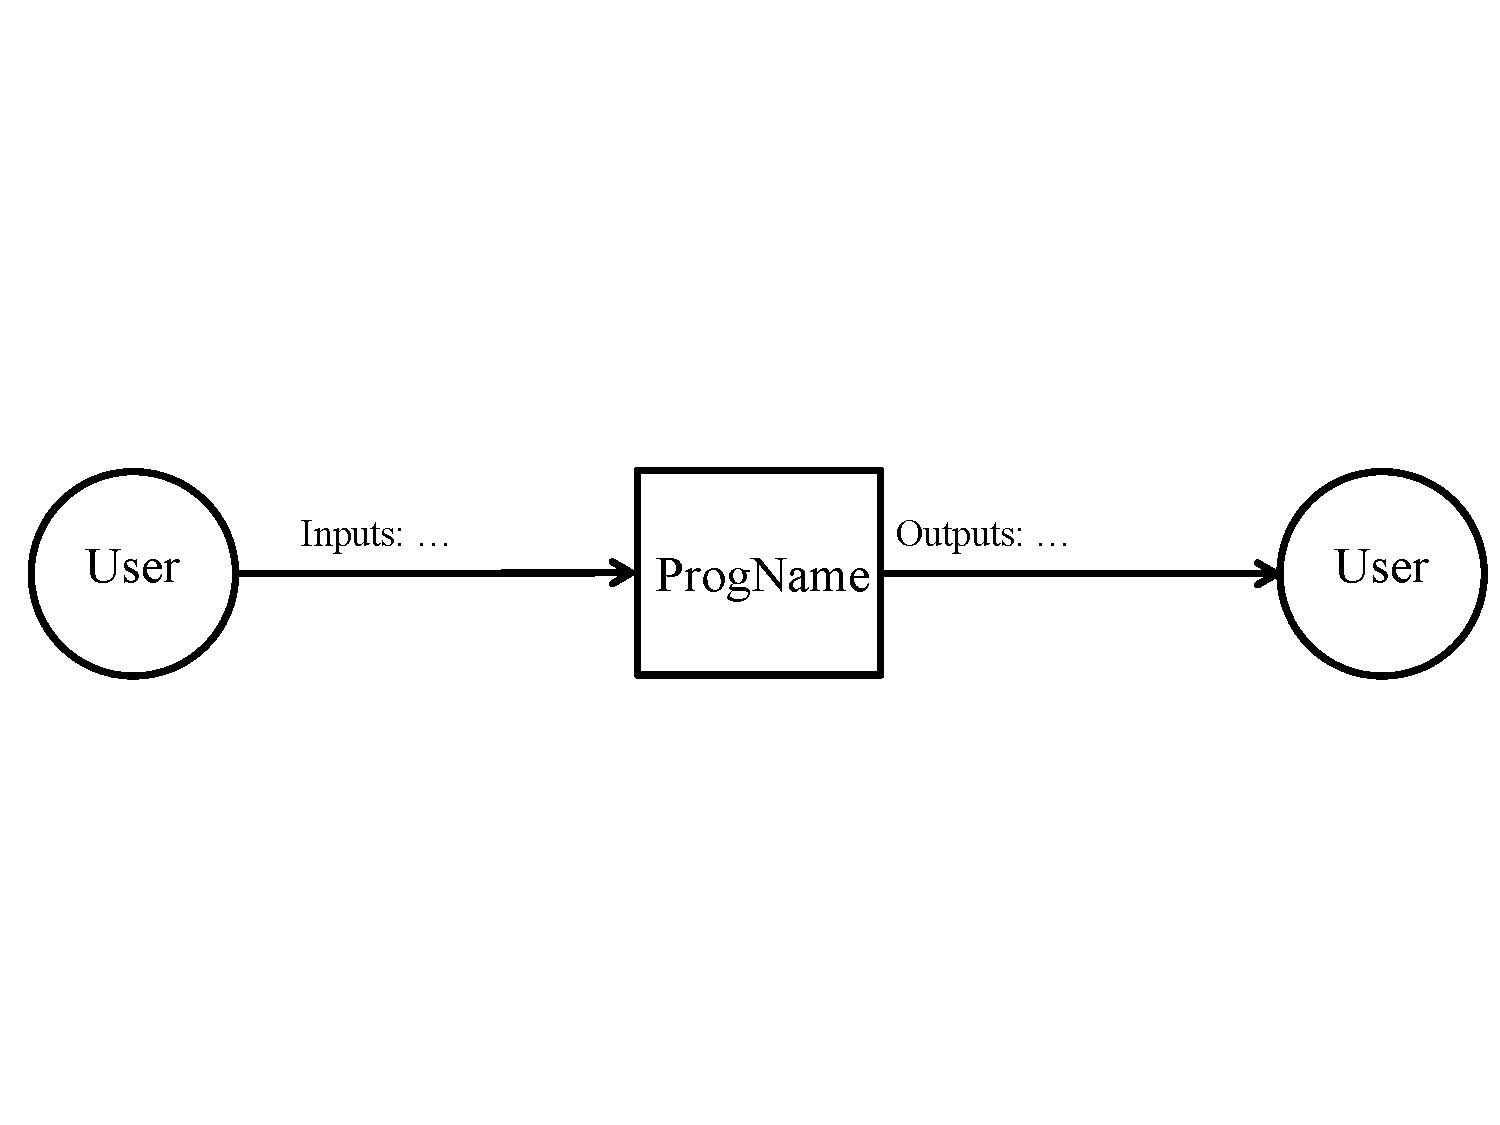
\includegraphics[width=0.6\textwidth]{SystemContextFigure}
%         \caption{System Context}
%         \label{Fig_SystemContext}
%     \end{center}
% \end{figure}

\begin{figure}[h!]
    \begin{center}
        \begin{tikzpicture}
            \node [draw,circle] (I) at (-6, 0) {\textbf{User}};
            \node [draw,rectangle] (BB) at (0, 0) {\textbf{BeamBending}};
            \node [draw,circle] (O) at (6, 0) {\textbf{User}};

            \draw [thick,->] (I) -- (BB) node[midway,above] {\parbox{3cm}{\center\textbf{Input}:\newline{} beam \& load specifications.}};
            \draw [thick,->] (BB) -- (O) node[midway,above] {\parbox{3cm}{\center\textbf{Output}:\newline{} deflection curve.}};
        \end{tikzpicture}
    \end{center}
    \caption{System Context}
    \label{Fig_SystemContext}
\end{figure}

\begin{itemize}
    \item User Responsibilities:
          \begin{itemize}

              \item Providing material properties of the beam, taking required
                    units, assumptions, and applicability of the beam into
                    consideration.

              \item Providing an explanation of the imposed load as a function
                    of the distance from the leftward pinned support.

              \item Interpret the output of the program taking this SRS document
                    into consideration and use an audited and reliable copy of a
                    software related to this SRS.

          \end{itemize}

    \item \progname{} Responsibilities:
          \begin{itemize}

              \item Detect data type mismatches, such as a string of characters
                    instead of a floating point number.

              \item Evaluate applicability of the input arguments to the
                    proposed ``solution'' outlined in this document, such as
                    numbers being above a certain threshold with respect to
                    others (e.g., the number of sampling points must be a
                    positive, non-zero, number).

              \item Calculate the imposed loading and resultant deflection at
                    every desired sampling point, the angles of rotation between
                    the beam and the respective supports, the force reactions at
                    the supports, and the movement of the beam in the horizontal
                    direction.

          \end{itemize}
\end{itemize}

\subsection{User Characteristics} \label{SecUserCharacteristics}

The user of this software should be a civil engineer or equivalent, and have a
working understanding of the deflection of beams, shear forces, bending moments,
and related concepts. If applied in educational purposes, only an understanding
of first-year physics and calculus is required to generally understand the
program and simulate a simply-supported beam across various scenarios.

\subsection{System Constraints}

The final software should be built using Drasil to encode the problem and
generate a problem using a Boundary Value Problem (BVP) solver. There are no
other system constraints.

\newpage

%%%%%%%%%%%%%%%%%%%%%%%%%%%%%%%%%%%%%%%%%%%%%%%%%%%%%%%%%%%%%%%%%%%%%%%%%%%%%%%
% Specific System Description
%%%%%%%%%%%%%%%%%%%%%%%%%%%%%%%%%%%%%%%%%%%%%%%%%%%%%%%%%%%%%%%%%%%%%%%%%%%%%%%

\section{Specific System Description} \label{sec_ssd}

This section first presents the problem description, which gives a high-level
view of the problem to be solved.  This is followed by the solution characteristics
specification, which presents the assumptions, theories, definitions and finally
the instance models.  \plt{Add any project specific details that are relevant
    for the section overview.}

\subsection{Problem Description} \label{Sec_pd}

\progname{} is intended to solve for the deflection a beam experiences given a
load-application function and properties of the beam.

\subsubsection{Terminology and  Definitions}

\plt{This section is expressed in words, not with equations.  It provide the
    meaning of the different words and phrases used in the domain of the problem.
    The terminology is used to introduce concepts from the world outside of the
    mathematical model  The terminology provides a real world connection to give the
    mathematical model meaning.}

This subsection provides a list of terms that are used in the subsequent
sections and their meaning, with the purpose of reducing ambiguity and making it
easier to correctly understand the requirements:

\an{I need to add in the definitions.}

\begin{itemize}

    \item Deflection:

    \item Shear force:

    \item Bending moment:

    \item Load:

    \item Beam:

    \item Simply supported beam:

    \item Pinned support:

    \item Roller support:

    \item Young's modulus:

    \item Moment of inertia:

\end{itemize}

\subsubsection{Physical System Description} \label{sec_phySystDescrip}

\begin{figure}[H]
    \begin{center}
        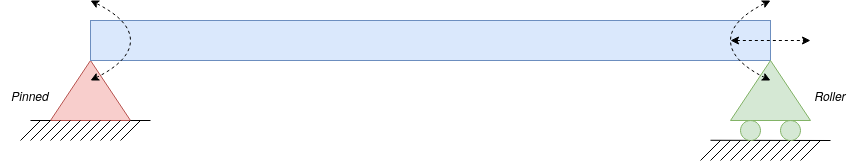
\includegraphics[width=0.9\textwidth]{temp/beam_bending_diagram.drawio.png}
        \caption{\label{beam_bending_diagram} Diagram of a Simply Supported Beam}
    \end{center}
\end{figure}

\plt{The purpose of this section is to clearly and unambiguously state the
    physical system that is to be modelled. Effective problem solving requires a
    logical and organized approach. The statements on the physical system to be
    studied should cover enough information to solve the problem. The physical
    description involves element identification, where elements are defined as
    independent and separable items of the physical system. Some example elements
    include acceleration due to gravity, the mass of an object, and the size and
    shape of an object. Each element should be identified and labelled, with their
    interesting properties specified clearly. The physical description can also
    include interactions of the elements, such as the following: i) the
    interactions between the elements and their physical environment; ii) the
    interactions between elements; and, iii) the initial or boundary conditions.}

The physical system of \progname{}, as shown in
\Cref{beam_bending_diagram_annotated}, includes the following elements:

\begin{itemize}

    \item[PS1:] a slender beam,

    \item[PS2:] a pinned support,

    \item[PS3:] a roller support, and

    \item[PS4:] an applied load, with load across points captured by a function.

\end{itemize}

\begin{figure}[H]
    \begin{center}
        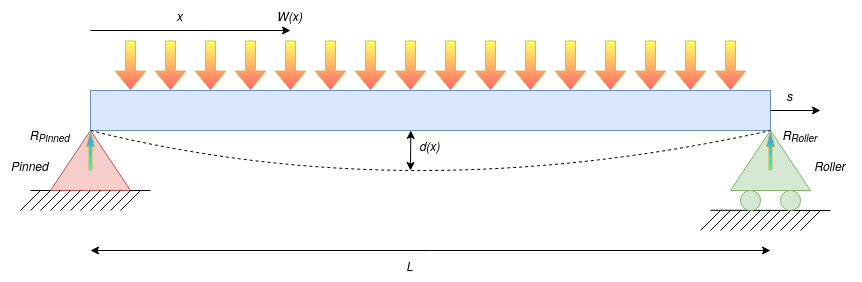
\includegraphics[width=0.9\textwidth]{temp/beam_bending_diagram_annotated.drawio.png}
        \caption{\label{beam_bending_diagram_annotated} Diagram of a Simply Supported Beam Under Load}
    \end{center}
\end{figure}

\subsubsection{Goal Statements} \label{sssec_goals}

\noindent Given the (constant) length, modulus of elasticity, and moment of
inertia across cross-sections for the beam, and the applied load on the beam as
a function from the distance of the leftward pinned support, the goal statements
are:

\begin{itemize}

    \item[GS\refstepcounter{goalnum}\thegoalnum \label{deflection}:] Calculate
        the deflection of the beam across $n+1$ equally spaced samples.

    \item[GS\refstepcounter{goalnum}\thegoalnum \label{res}:] Coupled together,
        calculate the deflection of the beam across $n+1$ equally spaced samples
        with the related applied load at that same sampled point.

\end{itemize}

\an{I'm not sure if I should also work to capture the shear force and bending
    moment diagrams too.}

\subsection{Solution Characteristics Specification}

\plt{This section specifies the information in the solution domain of the system
    to be developed. This section is intended to express what is required in
    such a way that analysts and stakeholders get a clear picture, and the
    latter will accept it. The purpose of this section is to reduce the problem
    into one expressed in mathematical terms. Mathematical expertise is used to
    extract the essentials from the underlying physical description of the
    problem, and to collect and substantiate all physical data pertinent to the
    problem.}

\plt{This section presents the solution characteristics by successively refining
    models.  It starts with the abstract/general Theoretical Models (TMs) and
    refines them to the concrete/specific Instance Models (IMs).  If necessary
    there are intermediate refinements to General Definitions (GDs).  All of these
    refinements can potentially use Assumptions (A) and Data Definitions (DD).
    TMs are refined to create new models, that are called GMs or IMs. DDs are not
    refined; they are just used. GDs and IMs are derived, or refined, from other
    models. DDs are not derived; they are just given. TMs are also just given, but
    they are refined, not used.  If a potential DD includes a derivation, then
    that means it is refining other models, which would make it a GD or an IM.}

\plt{The above makes a distinction between ``refined'' and ``used.'' A model is
    refined to another model if it is changed by the refinement. When we change a
    general 3D equation to a 2D equation, we are making a refinement, by applying
    the assumption that the third dimension does not matter. If we use a
    definition, like the definition of density, we aren't refining, or changing
    that definition, we are just using it.}

\plt{The same information can be a TM in one problem and a DD in another.  It is
    about how the information is used.  In one problem the definition of
    acceleration can be a TM, in another it would be a DD.}

\plt{There is repetition between the information given in the different chunks
    (TM, GDs etc) with other information in the document.  For instance, the
    meaning of the symbols, the units etc are repeated.  This is so that the
    chunks can stand on their own when being read by a reviewer/user.  It also
    facilitates reuse of the models in a different context.}

\noindent \plt{The relationships between the parts of the document are show in
    the following figure.  In this diagram ``may ref'' has the same role as
    ``uses'' above.  The figure adds ``Likely Changes,'' which are able to
    reference (use) Assumptions.}

\begin{figure}[H]
    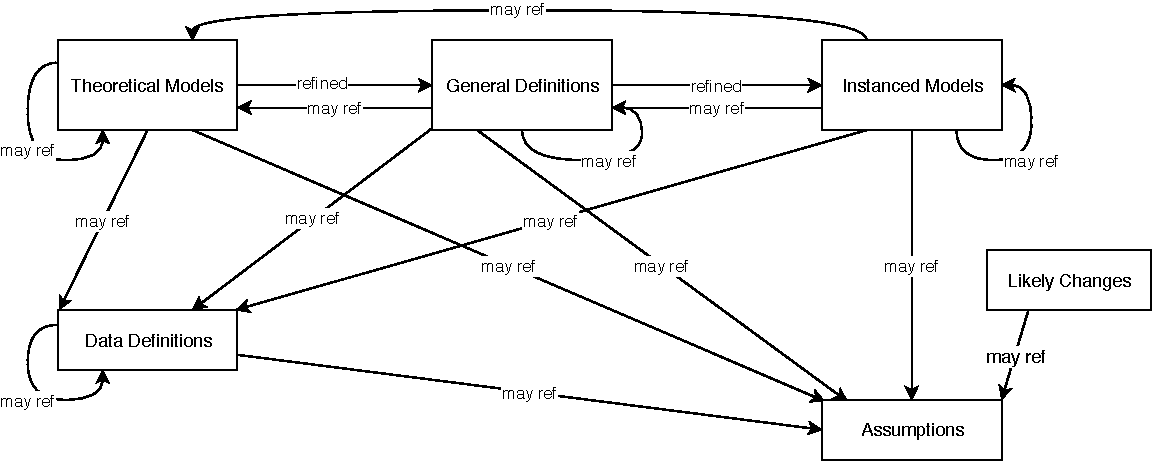
\includegraphics[scale=0.9]{RelationsBetweenTM_GD_IM_DD_A.pdf}
\end{figure}

The instance models that govern \progname{} are presented in
Subsection~\ref{sec_instance}.  The information to understand the meaning of the
instance models and their derivation is also presented, so that the instance
models can be verified.

\subsubsection{Assumptions} \label{sec_assumpt}

\plt{The assumptions are a refinement of the scope.  The scope is general, where
    the assumptions are specific.  All assumptions should be listed, even those
    that domain experts know so well that they are rarely (if ever) written down.}
\plt{The document should not take for granted that the reader knows which
    assumptions have been made. In the case of unusual assumptions, it is
    recommended that the documentation either include, or point to, an explanation
    and justification for the assumption.}

This section simplifies the original problem and helps in developing the
theoretical model by filling in the missing information for the physical
system. The numbers given in the square brackets refer to the theoretical model
    [T], general definition [GD], data definition [DD], instance model [IM], or
likely change [LC], in which the respective assumption is used.

\begin{itemize}

    \item[A\refstepcounter{assumpnum}\theassumpnum \label{A_meaningfulLabel}:]
        \plt{Short description of each assumption.  Each assumption
            should have a meaningful label.  Use cross-references to identify the
            appropriate traceability to T, GD, DD etc., using commands like dref, ddref
            etc.  Each assumption should be atomic - that is, there should not be an
            explicit (or implicit) ``and'' in the text of an assumption.}

\end{itemize}

\begin{itemize}
    \item Prismatic beam (straight, flat beam with a uniform cross-section),
    \item Slender beam (such that Euler-Bernoulli applies, 10:1 ratio of length
          to width),
    \item Constant modulus of elasticity and moment of inertia.
    \item ...
\end{itemize}

\subsubsection{Theoretical Models}\label{sec_theoretical}

\plt{Theoretical models are sets of abstract mathematical equations or axioms
    for solving the problem described in Section ``Physical System Description''
    (Section~\ref{sec_phySystDescrip}). Examples of theoretical models are
    physical laws, constitutive equations, relevant conversion factors, etc.}

This section focuses on the general equations and laws that \progname{} is based
on.  \plt{Modify the examples below for your problem, and add additional models
    as appropriate.}

~\newline

\an{I can make this theory a refinment of the more general 2nd-order ``curvature
    of an elastic beam'' equation. I'm not yet sure what I should define that as
    a refinement of yet, nor how far ``up'' I should go.}

\noindent
\deftheory
% #2 refname of theory
{TM:EBBDE}
% #3 label
{Euler-Bernoulli Beam Deflection Equation}
% #4 equation
{
    \(EI\frac{d^{4}y}{dx^{4}}=w(x)\)
}
% #5 description
{ The above equation describes the relationship between a beam's deflection
    (\(y(x)\)) and the applied load (\(w(x)\)) for any point along the beam (\(x\)).
    \an{Describe requirements and their relationship to the assumptions.}
}
% #6 Notes
{
    None.
}
% #7 Source
{
    \cite{EulerBernoulliWiki}
}
% #8 Referenced by
{
    \dref{ROCT}
}
% #9 Preconditions
{
    None
}
% #1 derivation - not applicable by default
{}

\plt{``Ref.\ By'' is used repeatedly with the different types of information.
    This stands for Referenced By.  It means that the models, definitions and
    assumptions listed reference the current model, definition or assumption.
    This information is given for traceability.  Ref. By provides a pointer in the
    opposite direction to what we commonly do.  You still need to have a reference
    in the other direction pointing to the current model, definition or
    assumption.  As an example, if T1 is referenced by G2, that means that G2 will
    explicitly include a reference to T1.}

~\newline

\subsubsection{General Definitions}\label{sec_gendef}

\plt{General Definitions (GDs) are a refinement of one or more TMs, and/or of
    other GDs.  The GDs are less abstract than the TMs.  Generally the reduction
    in abstraction is possible through invoking (using/referencing) Assumptions.
    For instance, the TM could be Newton's Law of Cooling stated abstracting.  The
    GD could take the general law and apply it to get a 1D equation.}

This section collects the laws and equations that will be used in building the
instance models.

\plt{Some projects may not have any content for this section, but the section
    heading should be kept.}

\plt{Modify the examples below for your problem, and add additional definitions
    as appropriate.}

~\newline

\noindent
\begin{minipage}{\textwidth}
    \renewcommand*{\arraystretch}{1.5}
    \begin{tabular}{| p{\colAwidth} | p{\colBwidth}|}
        \hline
        \rowcolor[gray]{0.9}
        Number      & GD\refstepcounter{defnum}\thedefnum \label{NL}                                     \\
        \hline
        Label       & \bf Newton's law of cooling                                                        \\
        \hline
        % Units&$MLt^{-3}T^0$\\
        % \hline
        SI Units    & \si{\watt\per\square\metre}                                                        \\
        \hline
        Equation    & $ q(t) = h \Delta T(t)$                                                            \\
        \hline
        Description &
        Newton's law of cooling describes convective cooling from a surface.  The law is
        stated as: the rate of heat loss from a body is proportional to the difference
        in temperatures between the body and its surroundings.
        \\
                    & $q(t)$ is the thermal flux (\si{\watt\per\square\metre}).                          \\
                    & $h$ is the heat transfer coefficient, assumed independent of $T$ (\aref{A_hcoeff})
        (\si{\watt\per\square\metre\per\celsius}).                                                       \\
                    & $\Delta T(t)$= $T(t) - T_{\text{env}}(t)$ is the time-dependent thermal gradient
        between the environment and the object (\si{\celsius}).
        \\
        \hline
        Source      & Citation here                                                                      \\
        \hline
        Ref.\ By    & \ddref{FluxCoil}, \ddref{FluxPCM}                                                  \\
        \hline
    \end{tabular}
\end{minipage}\\

\subsubsection*{Detailed derivation of simplified rate of change of temperature}

\plt{This may be necessary when the necessary information does not fit in the
    description field.}
\plt{Derivations are important for justifying a given GD.  You want it to be
    clear where the equation came from.}

\subsubsection{Data Definitions}\label{sec_datadef}

\plt{The Data Definitions are definitions of symbols and equations that are
    given for the problem.  They are not derived; they are simply used by other
    models.  For instance, if a problem depends on density, there may be a data
    definition for the equation defining density.  The DDs are given information
    that you can use in your other modules.}

\plt{All Data Definitions should be used (referenced) by at least one other
    model.}

This section collects and defines all the data needed to build the instance
models. The dimension of each quantity is also given.  \plt{Modify the examples
    below for your problem, and add additional definitions as appropriate.}

~\newline

\noindent
\begin{minipage}{\textwidth}
    \renewcommand*{\arraystretch}{1.5}
    \begin{tabular}{| p{\colAwidth} | p{\colBwidth}|}
        \hline
        \rowcolor[gray]{0.9}
        Number      & DD\refstepcounter{datadefnum}\thedatadefnum \label{FluxCoil} \\
        \hline
        Label       & \bf Heat flux out of coil                                    \\
        \hline
        Symbol      & $q_C$                                                        \\
        \hline
        % Units& $Mt^{-3}$\\
        % \hline
        SI Units    & \si{\watt\per\square\metre}                                  \\
        \hline
        Equation    & $q_C(t) = h_C (T_C - T_W(t))$, over area $A_C$               \\
        \hline
        Description &
        $T_C$ is the temperature of the coil (\si{\celsius}).  $T_W$ is the temperature of the water (\si{\celsius}).
        The heat flux out of the coil, $q_C$ (\si{\watt\per\square\metre}), is found by
        assuming that Newton's Law
        of Cooling applies (\aref{A_Newt_coil}).  This law (\dref{NL}) is used on the surface of
        the coil, which has area $A_C$ (\si{\square\metre}) and heat
        transfer coefficient $h_C$
        (\si{\watt\per\square\metre\per\celsius}).  This equation
        assumes that the temperature of the coil is constant over time (\aref{A_tcoil}) and that it does not vary along the length
        of the coil (\aref{A_tlcoil}).
        \\
        \hline
        Sources     & Citation here                                                \\
        \hline
        Ref.\ By    & \iref{ewat}                                                  \\
        \hline
    \end{tabular}
\end{minipage}\\

\subsubsection{Data Types}\label{sec_datatypes}

\plt{This section is optional.  In many scientific computing programs it isn't
    necessary, since the inputs and outpus are straightforward types, like reals,
    integers, and sequences of reals and integers.  However, for some problems it
    is very helpful to capture the type information.}

\plt{The data types are not derived; they are simply stated and used by other
    models.}

\plt{All data types must be used by at least one of the models.}

\plt{For the mathematical notation for expressing types, the recommendation is
    to use the notation of~\cite{HoffmanAndStrooper1995}.}

This section collects and defines all the data types needed to document the
models. \plt{Modify the examples below for your problem, and add additional
    definitions as appropriate.}

~\newline

\noindent
\begin{minipage}{\textwidth}
    \renewcommand*{\arraystretch}{1.5}
    \begin{tabular}{| p{\colAwidth} | p{\colBwidth}|}
        \hline
        \rowcolor[gray]{0.9}
        Type Name   & Name for Type                                              \\
        \hline
        Type Def    & mathematical definition of the type                        \\
        \hline
        Description & description here
        \\
        \hline
        Sources     & Citation here, if the type is borrowed from another source \\
        \hline
    \end{tabular}
\end{minipage}\\

\subsubsection{Instance Models} \label{sec_instance}

\plt{The motivation for this section is to reduce the problem defined in
    ``Physical System Description'' (Section~\ref{sec_phySystDescrip}) to one
    expressed in mathematical terms. The IMs are built by refining the TMs and/or
    GDs.  This section should remain abstract.  The SRS should specify the
    requirements without considering the implementation.}

This section transforms the problem defined in Section~\ref{Sec_pd} into
one which is expressed in mathematical terms. It uses concrete symbols defined
in Section~\ref{sec_datadef} to replace the abstract symbols in the models
identified in Sections~\ref{sec_theoretical} and~\ref{sec_gendef}.

The goals \plt{reference your goals} are solved by \plt{reference your instance
    models}.  \plt{other details, with cross-references where appropriate.}
\plt{Modify the examples below for your problem, and add additional models as
    appropriate.}

~\newline

%Instance Model 1

\noindent
\begin{minipage}{\textwidth}
    \renewcommand*{\arraystretch}{1.5}
    \begin{tabular}{| p{\colAwidth} | p{\colBwidth}|}
        \hline
        \rowcolor[gray]{0.9}
        Number      & IM\refstepcounter{instnum}\theinstnum \label{ewat}                                                                            \\
        \hline
        Label       & \bf Sampled deflection fo the beam $T_W$                                                                                      \\
        \hline
        Input       & $L_B$, $E_B$, $f(x)$ from \iref{epcm}                                                                                         \\
        \hline
        Output      & \(\vec{res} = <y(0), y(\frac{L_B}{n}), y(2\frac{L_B}{n}), ..., y(n\frac{L_B}{n})>\), such that                                \\
                    & \(E_{B}I_{B}\frac{d^{4}y}{dx^{4}}=f(x)\) where \(y(0)=0\), \(\frac{dy}{dx}(0)=0\), \(y(L_B)=0\), and \(\frac{dy}{dx}(L_B)=0\) \\
        \hline
        Description & ... (\textit{mostly} generated by Drasil) ...                                                                                 \\
        \\
        \hline
        Sources     & Citation here                                                                                                                 \\
        \hline
        Ref.\ By    & \iref{epcm}                                                                                                                   \\
        \hline
    \end{tabular}
\end{minipage}\\

%~\newline

\subsubsection*{Derivation of ...}

\plt{The derivation shows how the IM is derived from the TMs/GDs.  In cases
    where the derivation cannot be described under the Description field, it will
    be necessary to include this subsection.}

\subsubsection{Input Data Constraints} \label{sec_DataConstraints}

Table~\ref{TblInputVar} shows the data constraints on the input output
variables.  The column for physical constraints gives the physical limitations
on the range of values that can be taken by the variable.  The column for
software constraints restricts the range of inputs to reasonable values.  The
software constraints will be helpful in the design stage for picking suitable
algorithms.  The constraints are conservative, to give the user of the model the
flexibility to experiment with unusual situations.  The column of typical values
is intended to provide a feel for a common scenario.  The uncertainty column
provides an estimate of the confidence with which the physical quantities can be
measured.  This information would be part of the input if one were performing an
uncertainty quantification exercise.

The specification parameters in Table~\ref{TblInputVar} are listed in
Table~\ref{TblSpecParams}.

\begin{table}[!h]
    \caption{Input Variables} \label{TblInputVar}
    \renewcommand{\arraystretch}{1.2}
    \noindent \begin{longtable*}{l l l l c}
        \toprule
        \textbf{Var} & \textbf{Physical Constraints} & \textbf{Software Constraints} &
        \textbf{Typical Value} & \textbf{Uncertainty}\\
        \midrule
        $L$ & $L > 0$ & $L_{\text{min}} \leq L \leq L_{\text{max}}$ & 1.5 \si[per-mode=symbol] {\metre} & 10\%
        \\
        \bottomrule
    \end{longtable*}
\end{table}

\noindent
\begin{description}
    \item[(*)] \plt{you might need to add some notes or clarifications}
\end{description}

\begin{table}[!h]
    \caption{Specification Parameter Values} \label{TblSpecParams}
    \renewcommand{\arraystretch}{1.2}
    \noindent \begin{longtable*}{l l}
        \toprule
        \textbf{Var} & \textbf{Value} \\
        \midrule
        $L_\text{min}$ & 0.1 \si{\metre}\\
        \bottomrule
    \end{longtable*}
\end{table}

\subsubsection{Properties of a Correct Solution} \label{sec_CorrectSolution}

\noindent
A correct solution must exhibit \plt{fill in the details}.  \plt{These
    properties are in addition to the stated requirements.  There is no need to
    repeat the requirements here.  These additional properties may not exist for
    every problem.  Examples include conservation laws (like conservation of
    energy or mass) and known constraints on outputs, which are usually summarized
    in tabular form.  A sample table is shown in Table~\ref{TblOutputVar}}

\begin{table}[!h]
    \caption{Output Variables} \label{TblOutputVar}
    \renewcommand{\arraystretch}{1.2}
    \noindent \begin{longtable*}{l l}
        \toprule
        \textbf{Var} & \textbf{Physical Constraints} \\
        \midrule
        $T_W$ & $T_\text{init} \leq T_W \leq T_C$ (by~\aref{A_charge})
        \\
        \bottomrule
    \end{longtable*}
\end{table}

\plt{This section is not for test cases or techniques for verification and
    validation.  Those topics will be addressed in the Verification and Validation
    plan.}


%%%%%%%%%%%%%%%%%%%%%%%%%%%%%%%%%%%%%%%%%%%%%%%%%%%%%%%%%%%%%%%%%%%%%%%%%%%%%%%
% Requirements
%%%%%%%%%%%%%%%%%%%%%%%%%%%%%%%%%%%%%%%%%%%%%%%%%%%%%%%%%%%%%%%%%%%%%%%%%%%%%%%

\section{Requirements}

\plt{The requirements refine the goal statement.  They will make heavy use of
    references to the instance models.}

This section provides the functional requirements, the business tasks that the
software is expected to complete, and the nonfunctional requirements, the
qualities that the software is expected to exhibit.

\subsection{Functional Requirements}

\noindent \begin{itemize}

    \item[R\refstepcounter{reqnum}\thereqnum \label{R_Inputs}:] \plt{Requirements
            for the inputs that are supplied by the user.  This information has to be
            explicit.}

    \item[R\refstepcounter{reqnum}\thereqnum \label{R_OutputInputs}:] \plt{It isn't
            always required, but often echoing the inputs as part of the output is a
            good idea.}

    \item[R\refstepcounter{reqnum}\thereqnum \label{R_Calculate}:] \plt{Calculation
            related requirements.}

    \item[R\refstepcounter{reqnum}\thereqnum \label{R_VerifyOutput}:]
        \plt{Verification related requirements.}

    \item[R\refstepcounter{reqnum}\thereqnum \label{R_Output}:] \plt{Output related
            requirements.}

\end{itemize}

\plt{Every IM should map to at least one requirement, but not every requirement
    has to map to a corresponding IM.}

\subsection{Nonfunctional Requirements}

\plt{List your nonfunctional requirements.  You may consider using a fit
    criterion to make them verifiable.}
\plt{The goal is for the nonfunctional requirements to be unambiguous, abstract
    and verifiable.  This isn't easy to show succinctly, so a good strategy may be
    to give a ``high level'' view of the requirement, but allow for the details to
    be covered in the Verification and Validation document.}
\plt{An absolute requirement on a quality of the system is rarely needed.  For
    instance, an accuracy of 0.0101 \% is likely fine, even if the requirement is
    for 0.01 \% accuracy.  Therefore, the emphasis will often be more on
    describing now well the quality is achieved, through experimentation, and
    possibly theory, rather than meeting some bar that was defined a priori.}
\plt{You do not need an entry for correctness in your NFRs.  The purpose of the
    SRS is to record the requirements that need to be satisfied for correctness.
    Any statement of correctness would just be redundant. Rather than discuss
    correctness, you can characterize how far away from the correct (true)
    solution you are allowed to be.  This is discussed under accuracy.}

\noindent \begin{itemize}

    \item[NFR\refstepcounter{nfrnum}\thenfrnum \label{NFR_Accuracy}:]
        \textbf{Accuracy} \plt{Characterize the accuracy by giving the context/use for
            the software.  Maybe something like, ``The accuracy of the computed
            solutions should meet the level needed for $<$engineering or scientific
            application$>$.  The level of accuracy achieved by \progname{} shall be
            described following the procedure given in Section~X of the Verification and
            Validation Plan.''  A link to the VnV plan would be a nice extra.}

    \item[NFR\refstepcounter{nfrnum}\thenfrnum \label{NFR_Usability}:] \textbf{Usability}
        \plt{Characterize the usability by giving the context/use for the software.
            You should likely reference the user characteristics section.  The level of
            usability achieved by the software shall be described following the
            procedure given in Section~X of the Verification and Validation Plan.  A
            link to the VnV plan would be a nice extra.}

    \item[NFR\refstepcounter{nfrnum}\thenfrnum \label{NFR_Maintainability}:]
        \textbf{Maintainability} \plt{The effort required to make any of the likely
            changes listed for \progname{} should be less than FRACTION of the original
            development time.  FRACTION is then a symbolic constant that can be defined
            at the end of the report.}

    \item[NFR\refstepcounter{nfrnum}\thenfrnum \label{NFR_Portability}:]
        \textbf{Portability} \plt{This NFR is easier to write than the others.  The
            systems that \progname{} should run on should be listed here.  When possible
            the specific versions of the potential operating environments should be
            given.  To make the NFR verifiable a statement could be made that the tests
            from a given section of the VnV plan can be successfully run on all of the
            possible operating environments.}

    \item Other NFRs that might be discussed include verifiability,
          understandability and reusability.

\end{itemize}


%%%%%%%%%%%%%%%%%%%%%%%%%%%%%%%%%%%%%%%%%%%%%%%%%%%%%%%%%%%%%%%%%%%%%%%%%%%%%%%
% Likely Changes
%%%%%%%%%%%%%%%%%%%%%%%%%%%%%%%%%%%%%%%%%%%%%%%%%%%%%%%%%%%%%%%%%%%%%%%%%%%%%%%

\section{Likely Changes}

\noindent \begin{itemize}

    \item[LC\refstepcounter{lcnum}\thelcnum\label{LC_meaningfulLabel}:] \plt{Give
            the likely changes, with a reference to the related assumption (aref), as appropriate.}

\end{itemize}

%%%%%%%%%%%%%%%%%%%%%%%%%%%%%%%%%%%%%%%%%%%%%%%%%%%%%%%%%%%%%%%%%%%%%%%%%%%%%%%
% Unlikely Changes
%%%%%%%%%%%%%%%%%%%%%%%%%%%%%%%%%%%%%%%%%%%%%%%%%%%%%%%%%%%%%%%%%%%%%%%%%%%%%%%

\section{Unlikely Changes}

\noindent \begin{itemize}

    \item[LC\refstepcounter{lcnum}\thelcnum\label{LC_meaningfulLabel}:] \plt{Give
            the unlikely changes.  The design can assume that the changes listed will
            not occur.}

\end{itemize}

%%%%%%%%%%%%%%%%%%%%%%%%%%%%%%%%%%%%%%%%%%%%%%%%%%%%%%%%%%%%%%%%%%%%%%%%%%%%%%%
% Traceability Matrices and Graphs
%%%%%%%%%%%%%%%%%%%%%%%%%%%%%%%%%%%%%%%%%%%%%%%%%%%%%%%%%%%%%%%%%%%%%%%%%%%%%%%

\section{Traceability Matrices and Graphs}

The purpose of the traceability matrices is to provide easy references on what
has to be additionally modified if a certain component is changed.  Every time a
component is changed, the items in the column of that component that are marked
with an ``X'' may have to be modified as well.  Table~\ref{Table:trace} shows the
dependencies of theoretical models, general definitions, data definitions, and
instance models with each other. Table~\ref{Table:R_trace} shows the
dependencies of instance models, requirements, and data constraints on each
other. Table~\ref{Table:A_trace} shows the dependencies of theoretical models,
general definitions, data definitions, instance models, and likely changes on
the assumptions.

\plt{You will have to modify these tables for your problem.}

\plt{The traceability matrix is not generally symmetric.  If GD1 uses A1, that
    means that GD1's derivation or presentation requires invocation of A1.  A1
    does not use GD1.  A1 is ``used by'' GD1.}

\plt{The traceability matrix is challenging to maintain manually.  Please do
    your best.  In the future tools (like Drasil) will make this much easier.}

\afterpage{
    \begin{landscape}
        \begin{table}[h!]
            \centering
            \begin{tabular}{|c|c|c|c|c|c|c|c|c|c|c|c|c|c|c|c|c|c|c|c|}
                \hline
                                    & \aref{A_OnlyThermalEnergy} & \aref{A_hcoeff} & \aref{A_mixed} & \aref{A_tpcm} & \aref{A_const_density} & \aref{A_const_C} & \aref{A_Newt_coil} & \aref{A_tcoil} & \aref{A_tlcoil} & \aref{A_Newt_pcm} & \aref{A_charge} & \aref{A_InitTemp} & \aref{A_OpRangePCM} & \aref{A_OpRange} & \aref{A_htank} & \aref{A_int_heat} & \aref{A_vpcm} & \aref{A_PCM_state} & \aref{A_Pressure} \\
                \hline
                \tref{T_COE}        & X                          &                 &                &               &                        &                  &                    &                &                 &                   &                 &                   &                     &                  &                &                   &               &                    &                   \\ \hline
                \tref{T_SHE}        &                            &                 &                &               &                        &                  &                    &                &                 &                   &                 &                   &                     &                  &                &                   &               &                    &                   \\ \hline
                \tref{T_LHE}        &                            &                 &                &               &                        &                  &                    &                &                 &                   &                 &                   &                     &                  &                &                   &               &                    &                   \\ \hline
                \dref{NL}           &                            & X               &                &               &                        &                  &                    &                &                 &                   &                 &                   &                     &                  &                &                   &               &                    &                   \\ \hline
                \dref{ROCT}         &                            &                 & X              & X             & X                      & X                &                    &                &                 &                   &                 &                   &                     &                  &                &                   &               &                    &                   \\ \hline
                \ddref{FluxCoil}    &                            &                 &                &               &                        &                  & X                  & X              & X               &                   &                 &                   &                     &                  &                &                   &               &                    &                   \\ \hline
                \ddref{FluxPCM}     &                            &                 & X              & X             &                        &                  &                    &                &                 & X                 &                 &                   &                     &                  &                &                   &               &                    &                   \\ \hline
                \ddref{D_HOF}       &                            &                 &                &               &                        &                  &                    &                &                 &                   &                 &                   &                     &                  &                &                   &               &                    &                   \\ \hline
                \ddref{D_MF}        &                            &                 &                &               &                        &                  &                    &                &                 &                   &                 &                   &                     &                  &                &                   &               &                    &                   \\ \hline
                \iref{ewat}         &                            &                 &                &               &                        &                  &                    &                &                 &                   & X               & X                 &                     & X                & X              & X                 &               &                    & X                 \\ \hline
                \iref{epcm}         &                            &                 &                &               &                        &                  &                    &                &                 &                   &                 & X                 & X                   &                  &                & X                 & X             & X                  &                   \\ \hline
                \iref{I_HWAT}       &                            &                 &                &               &                        &                  &                    &                &                 &                   &                 &                   &                     & X                &                &                   &               &                    & X                 \\ \hline
                \iref{I_HPCM}       &                            &                 &                &               &                        &                  &                    &                &                 &                   &                 &                   & X                   &                  &                &                   &               & X                  &                   \\ \hline
                \lcref{LC_tpcm}     &                            &                 &                & X             &                        &                  &                    &                &                 &                   &                 &                   &                     &                  &                &                   &               &                    &                   \\ \hline
                \lcref{LC_tcoil}    &                            &                 &                &               &                        &                  &                    & X              &                 &                   &                 &                   &                     &                  &                &                   &               &                    &                   \\ \hline
                \lcref{LC_tlcoil}   &                            &                 &                &               &                        &                  &                    &                & X               &                   &                 &                   &                     &                  &                &                   &               &                    &                   \\ \hline
                \lcref{LC_charge}   &                            &                 &                &               &                        &                  &                    &                &                 &                   & X               &                   &                     &                  &                &                   &               &                    &                   \\ \hline
                \lcref{LC_InitTemp} &                            &                 &                &               &                        &                  &                    &                &                 &                   &                 & X                 &                     &                  &                &                   &               &                    &                   \\ \hline
                \lcref{LC_htank}    &                            &                 &                &               &                        &                  &                    &                &                 &                   &                 &                   &                     &                  & X              &                   &               &                    &                   \\
                \hline
            \end{tabular}
            \caption{Traceability Matrix Showing the Connections Between Assumptions and Other Items}
            \label{Table:A_trace}
        \end{table}
    \end{landscape}
}

\begin{table}[h!]
    \centering
    \begin{tabular}{|c|c|c|c|c|c|c|c|c|c|c|c|c|c|c|c|c|c|c|c|c|c|c|c|}
        \hline
                         & \tref{T_COE} & \tref{T_SHE} & \tref{T_LHE} & \dref{NL} & \dref{ROCT} & \ddref{FluxCoil} & \ddref{FluxPCM} & \ddref{D_HOF} & \ddref{D_MF} & \iref{ewat} & \iref{epcm} & \iref{I_HWAT} & \iref{I_HPCM} \\
        \hline
        \tref{T_COE}     &              &              &              &           &             &                  &                 &               &              &             &             &               &               \\ \hline
        \tref{T_SHE}     &              &              & X            &           &             &                  &                 &               &              &             &             &               &               \\ \hline
        \tref{T_LHE}     &              &              &              &           &             &                  &                 &               &              &             &             &               &               \\ \hline
        \dref{NL}        &              &              &              &           &             &                  &                 &               &              &             &             &               &               \\ \hline
        \dref{ROCT}      & X            &              &              &           &             &                  &                 &               &              &             &             &               &               \\ \hline
        \ddref{FluxCoil} &              &              &              & X         &             &                  &                 &               &              &             &             &               &               \\ \hline
        \ddref{FluxPCM}  &              &              &              & X         &             &                  &                 &               &              &             &             &               &               \\ \hline
        \ddref{D_HOF}    &              &              &              &           &             &                  &                 &               &              &             &             &               &               \\ \hline
        \ddref{D_MF}     &              &              &              &           &             &                  &                 & X             &              &             &             &               &               \\ \hline
        \iref{ewat}      &              &              &              &           & X           & X                & X               &               &              &             & X           &               &               \\ \hline
        \iref{epcm}      &              &              &              &           & X           &                  & X               &               & X            & X           &             &               & X             \\ \hline
        \iref{I_HWAT}    &              & X            &              &           &             &                  &                 &               &              &             &             &               &               \\ \hline
        \iref{I_HPCM}    &              & X            & X            &           &             &                  & X               & X             & X            &             & X           &               &               \\
        \hline
    \end{tabular}
    \caption{Traceability Matrix Showing the Connections Between Items of Different Sections}
    \label{Table:trace}
\end{table}

\begin{table}[h!]
    \centering
    \begin{tabular}{|c|c|c|c|c|c|c|c|}
        \hline
                               & \iref{ewat} & \iref{epcm} & \iref{I_HWAT} & \iref{I_HPCM} & \ref{sec_DataConstraints} & \rref{R_RawInputs} & \rref{R_MassInputs} \\
        \hline
        \iref{ewat}            &             & X           &               &               &                           & X                  & X                   \\ \hline
        \iref{epcm}            & X           &             &               & X             &                           & X                  & X                   \\ \hline
        \iref{I_HWAT}          &             &             &               &               &                           & X                  & X                   \\ \hline
        \iref{I_HPCM}          &             & X           &               &               &                           & X                  & X                   \\ \hline
        \rref{R_RawInputs}     &             &             &               &               &                           &                    &                     \\ \hline
        \rref{R_MassInputs}    &             &             &               &               &                           & X                  &                     \\ \hline
        \rref{R_CheckInputs}   &             &             &               &               & X                         &                    &                     \\ \hline
        \rref{R_OutputInputs}  & X           & X           &               &               &                           & X                  & X                   \\ \hline
        \rref{R_TempWater}     & X           &             &               &               &                           &                    &                     \\ \hline
        \rref{R_TempPCM}       &             & X           &               &               &                           &                    &                     \\ \hline
        \rref{R_EnergyWater}   &             &             & X             &               &                           &                    &                     \\ \hline
        \rref{R_EnergyPCM}     &             &             &               & X             &                           &                    &                     \\ \hline
        \rref{R_VerifyOutput}  &             &             & X             & X             &                           &                    &                     \\ \hline
        \rref{R_timeMeltBegin} &             & X           &               &               &                           &                    &                     \\ \hline
        \rref{R_timeMeltEnd}   &             & X           &               &               &                           &                    &                     \\
        \hline
    \end{tabular}
    \caption{Traceability Matrix Showing the Connections Between Requirements and Instance Models}
    \label{Table:R_trace}
\end{table}

The purpose of the traceability graphs is also to provide easy references on
what has to be additionally modified if a certain component is changed.  The
arrows in the graphs represent dependencies. The component at the tail of an
arrow is depended on by the component at the head of that arrow. Therefore, if a
component is changed, the components that it points to should also be
changed. Figure~\ref{Fig_ATrace} shows the dependencies of theoretical models,
general definitions, data definitions, instance models, likely changes, and
assumptions on each other. Figure~\ref{Fig_RTrace} shows the dependencies of
instance models, requirements, and data constraints on each other.

% \begin{figure}[h!]
% 	\begin{center}
% 		%\rotatebox{-90}
% 		{
% 			\includegraphics[width=\textwidth]{ATrace.png}
% 		}
% 		\caption{\label{Fig_ATrace} Traceability Matrix Showing the Connections Between Items of Different Sections}
% 	\end{center}
% \end{figure}


% \begin{figure}[h!]
% 	\begin{center}
% 		%\rotatebox{-90}
% 		{
% 			\includegraphics[width=0.7\textwidth]{RTrace.png}
% 		}
% 		\caption{\label{Fig_RTrace} Traceability Matrix Showing the Connections Between Requirements, Instance Models, and Data Constraints}
% 	\end{center}
% \end{figure}

%%%%%%%%%%%%%%%%%%%%%%%%%%%%%%%%%%%%%%%%%%%%%%%%%%%%%%%%%%%%%%%%%%%%%%%%%%%%%%%
% Development Plan
%%%%%%%%%%%%%%%%%%%%%%%%%%%%%%%%%%%%%%%%%%%%%%%%%%%%%%%%%%%%%%%%%%%%%%%%%%%%%%%

\section{Development Plan}

\plt{This section is optional.  It is used to explain the plan for developing
    the software.  In particular, this section gives a list of the order in which
    the requirements will be implemented.  In the context of a course  this is
    where you can indicate which requirements will be implemented as part of the
    course, and which will be ``faked'' as future work.  This section can be
    organized as a prioritized list of requirements, or it could should the
    requirements that will be implemented for ``phase 1'', ``phase 2'', etc.}


%%%%%%%%%%%%%%%%%%%%%%%%%%%%%%%%%%%%%%%%%%%%%%%%%%%%%%%%%%%%%%%%%%%%%%%%%%%%%%%
% Values of Auxiliar Constants
%%%%%%%%%%%%%%%%%%%%%%%%%%%%%%%%%%%%%%%%%%%%%%%%%%%%%%%%%%%%%%%%%%%%%%%%%%%%%%%

\section{Values of Auxiliary Constants}

\plt{Show the values of the symbolic parameters introduced in the report.}

\plt{The definition of the requirements will likely call for SYMBOLIC\_CONSTANTS.
    Their values are defined in this section for easy maintenance.}

\plt{The value of FRACTION, for the Maintainability NFR would be given here.}

\newpage

%%%%%%%%%%%%%%%%%%%%%%%%%%%%%%%%%%%%%%%%%%%%%%%%%%%%%%%%%%%%%%%%%%%%%%%%%%%%%%%
% Bibliography
%%%%%%%%%%%%%%%%%%%%%%%%%%%%%%%%%%%%%%%%%%%%%%%%%%%%%%%%%%%%%%%%%%%%%%%%%%%%%%%

\printbibliography[heading=bibintoc]

\newpage

%%%%%%%%%%%%%%%%%%%%%%%%%%%%%%%%%%%%%%%%%%%%%%%%%%%%%%%%%%%%%%%%%%%%%%%%%%%%%%%
% Appendix
%%%%%%%%%%%%%%%%%%%%%%%%%%%%%%%%%%%%%%%%%%%%%%%%%%%%%%%%%%%%%%%%%%%%%%%%%%%%%%%

\newpage{}
\section*{Appendix --- Reflection}

The information in this section will be used to evaluate the team members on the
graduate attribute of Lifelong Learning.  Please answer the following questions:

\begin{enumerate}
    \item What knowledge and skills will the team collectively need to acquire to
          successfully complete this capstone project?  Examples of possible knowledge
          to acquire include domain specific knowledge from the domain of your
          application, or software engineering knowledge, mechatronics knowledge or
          computer science knowledge.  Skills may be related to technology, or writing,
          or presentation, or team management, etc.  You should look to identify at
          least one item for each team member.
    \item For each of the knowledge areas and skills identified in the previous
          question, what are at least two approaches to acquiring the knowledge or
          mastering the skill?  Of the identified approaches, which will each team
          member pursue, and why did they make this choice?
\end{enumerate}

\end{document}
